\documentclass{article}
\usepackage[utf8]{inputenc} %кодировка
\usepackage[T2A]{fontenc}
\usepackage[english,russian]{babel} %русификатор 
\usepackage{mathtools} %библиотека матеши
\usepackage[left=1cm,right=1cm,top=2cm,bottom=2cm,bindingoffset=0cm]{geometry} %изменение отступов на листе
\usepackage{amsmath}
\usepackage{graphicx} %библиотека для графики и картинок
\graphicspath{}
\DeclareGraphicsExtensions{.pdf,.png,.jpg}
\usepackage{subcaption}
\usepackage{pgfplots}
\usepackage{listings}
\usepackage{derivative}
\pgfplotsset{compat=1.16}

\begin{document}
% НАЧАЛО ТИТУЛЬНОГО ЛИСТА
\begin{center}
    \Large
    Федеральное государственное автономное \\
    образовательное учреждение высшего образования \\ 
    «Научно-образовательная корпорация ИТМО»\\
    \vspace{0.5cm}
    \large
    Факультет программной инженерии и компьютерной техники \\
    Направление подготовки 09.03.04 Программная инженерия \\
    \vspace{1cm}
    \Large
    \textbf{Отчёт по лабораторной работе №2} \\
    По дисциплине «Вычислительная математика» (четвёртый семестр)\\
    \large
    \vspace{8cm}

    \begin{minipage}{.33\textwidth}
    \end{minipage}
    \hfill
    \begin{minipage}{.4\textwidth}
    
        \textbf{Студент}: \vspace{.1cm} \\
        \ Дениченко Александр P3212\\
        \textbf{Практик}:  \\
        \ Наумова Надежда Александровна
    \end{minipage}
    \vfill
Санкт-Петербург\\ 2024 г.
\end{center}

% КОНЕЦ ТИТУЛЬНОГО ЛИСТА 
\newpage
\begin{center}
    \LARGE
    \color{pink}
    \LaTeX \color{lime}.
\end{center}

\section{Цель работы}

Изучить численные методы решения нелинейных уравнений и их
систем, найти корни заданного нелинейного уравнения/системы нелинейных уравнений,
выполнить программную реализацию методов.


\section{Задание}
Часть 1.

1. Отделить корни заданного нелинейного уравнения графически (вид уравнения представлен в табл. 6)

2. Определить интервалы изоляции корней.

3. Уточнить корни нелинейного уравнения (см. табл. 6) с точностью $\epsilon=10^{-2}$.

4. Используемые методы для уточнения каждого из 3-х корней многочлена
представлены в таблице 7.

5. Вычисления оформить в виде таблиц (1-5), в зависимости от заданного метода. Для всех значений в таблице удержать 3 знака после запятой.

5.1 Для метода половинного деления заполнить таблицу 1.

5.2 Для метода хорд заполнить таблицу 2.

5.3 Для метода Ньютона заполнить таблицу 3.

5.4 Для метода секущих заполнить таблицу 4.

5.5 Для метода простой итерации заполнить таблицу 5. Проверить условие сходимости метода на выбранном интервале.

6. Заполненные таблицы отобразить в отчете.
\\ \\
Вид нелинейного уравнения для вычислительной реализации:
\[
    3x^3+1,7x^2-15,42x+6,89\]
Выбор метода для вычислительной реализации задачи:
\begin{table}[h]
    \centering
    \begin{tabular}{|*{4}{c|}}
        \hline
        Номер & Крайний & Крайний & Центральный  \\
        варианта & правый корень & левый корень & корень \\
        \hline
        8 & Метод простой итерации (5) & Метод хорд (2) & Метод Ньютона (3) \\
        \hline
    \end{tabular}
    \caption{Методы для вычислительной реализации}
\end{table}

\section{Выполнение первой части}
Точки пересечения:

\[x_3(1.67953,0)\] 
\[x_2(0.498258,0)\] 
\[x_1(-2.7445,0)\]
Построим график функции:
\begin{center}
    \begin{tikzpicture}
        \begin{axis}[
            xlabel={$x$},
            ylabel={$y$},
            xmin=-4, xmax=4,
            ymin=-10, ymax=30,
            axis lines=middle,
            grid=both,
            samples=1000,
            domain=-4:4,
            thick,
            legend style={at={(0.5,-0.15)},anchor=north}
        ]
        
        \addplot[blue] {3*x^3 + 1.7*x^2 - 15.42*x + 6.89};
        \addlegendentry{$3x^3 + 1.7x^2 - 15.42x + 6.89$}
        % Находим корни уравнения
        \draw[fill=black] (1.67953,0) circle [radius=2pt] node[below] {$x_3$};
        \draw[fill=black] (0.498258,0) circle [radius=2pt] node[below] {$x_2$};
        \draw[fill=black] (-2.7445,0) circle [radius=2pt] node[below] {$x_1$};
        
        \end{axis}
        \end{tikzpicture}
\end{center}
\textbf{1. Метод простой итерации для $x_3(1.67953,0)$.}

\begin{center}
    \begin{tikzpicture}
        \begin{axis}[
            xlabel={$x$},
            ylabel={$y$},
            xmin=1.1, xmax=2,
            ymin=-5, ymax=2,
            axis lines=middle,
            grid=both,
            samples=500,
            domain=-4:4,
            thick,
            legend style={at={(0.5,-0.15)},anchor=north}
        ]
        
        \addplot[blue] {3*x^3 + 1.7*x^2 - 15.42*x + 6.89};
        \addlegendentry{$3x^3 + 1.7x^2 - 15.42x + 6.89$}
        % Находим корни уравнения
        \draw[fill=black] (1.67953,0) circle [radius=2pt] node[below] {$x_3$};
        \draw[fill=black] (0.498258,0) circle [radius=2pt] node[below] {$x_2$};
        \draw[fill=black] (-2.7445,0) circle [radius=2pt] node[below] {$x_1$};
        
        \end{axis}
        \end{tikzpicture}
\end{center}

Приведём уравнение:
\[
    3x^3+1,7x^2-15,42x+6,89 = 0 \]
к следующему виду:
\[x = \phi (x)\]
получим:
\[
    \phi (x) = 0,195x^3+0,110x^2+0,447 = 0 \]
    \[
    \phi' (x) = 0,585x^2+0,220x \]
Пусть начальное приближение будет:
\[
    a_0 = 1,2;\ b_0 = 2\]
Тогда проверим условие сходимости:
\[
    \phi' (1,2) = 0,805 < 1 \]
    \[
    \phi' (2) = 0,585\cdot 4+0,220\cdot 2 = 2,34+0,44 = 2,78 > 1 \]
\[
    q = max_{[a,b]}|\phi'(x)| = 2,78 > 1
\]
Сходимости нет.
\\ \\
Пойдём по другому способу, где применяется приём введения параметра $\lambda$:
\[
    f(x) = 3x^3+1,7x^2-15,42x+6,89 \]
\[\lambda f(x) = 0\ (\lambda!=0)\]
\[\phi(x)\ = x+ \lambda f(x) \]
\[\phi'(x)\ = 1+ \lambda f'(x) \]
\[f'(x) = 9x^2 +3,4x - 15,42\]
\[f'(1,2) = 9\cdot (1,2)^2 +3,4\cdot (1,2) - 15,42 = 1,62\]
\[f'(2) = 9\cdot 4 +3,4\cdot 2 - 15,42 = 27,38\]
Так как $f'[a, b] > 0$, то рассматриваем:
\[
    \lambda = - \frac{1}{max|f'(x)|} = -\frac{1}{27,38} = -0,037\] 
Подставим:
\[\phi(x) = x -0,037 \cdot (3x^3+1,7x^2-15,42x+6,89)= \] 
\[= 1,571x - 0,111x^3 - 0,063x^2 - 0,255\]
\[\phi'(x) = 1,571 - 0,333 x^2 - 0,126x\]
Проверим точки:
\[\phi'(1,2) = 1,571 - 0,333\cdot(1,2)^2 - 0,126\cdot 1,2 = 0,940 < 1\]
\[\phi'(2) = 1,571 - 0,333\cdot(2)^2 - 0,126\cdot 2 = -0,013 < 1\]
Условие сходимости выполняется!
\[x_0 = 1,2 \]
\[x_1 = \phi(x_0) = 1,571\cdot 1,2 - 0,111\cdot(1,2)^3 - 0,063\cdot(1,2)^2 - 0,255 = 1,348\]
\[x_2 = 1,571\cdot 1,348 - 0,111\cdot(1,348)^3 - 0,063\cdot(1,348)^2 - 0,255 = 1,476\] 
\[f(x_2) = 3\cdot (1,476)^3+1,7\cdot (1,476)^2-15,42\cdot (1,476)+6,89 = -2,520\]
...
\[
    f(x) = 3x^3+1,7x^2-15,42x+6,89 \]
\[\phi(x)= 1,571x - 0,111x^3 - 0,063x^2 - 0,255\]


\begin{table}[h]
    \centering
    \begin{tabular}{|*{6}{c|}}
        \hline
        Номер & $x_i$ & $x_{i+1}$ & $\phi(x_{i+1})$& $f(x_{i+1})$& $|x_{i+1} - x_i|$  \\
        \hline
        0& 1,2& 1,348& 1,476&-2,520& 0,148\\
        \hline
        1& 1,348& 1,476& 1,57& -2,520& 0,128\\
        \hline
        2& 1,476& 1,57& 1,627&-1,519& 0,094\\
        \hline
        3& 1,57& 1,627& 1,656& -0,778&0,057\\
        \hline
        4& 1,627& 1,656& 1,67& -0,36& 0,029\\
        \hline
        5& 1,656& 1,67& 1,676& -0,148& 0,014\\
        \hline
        6& 1,67& 1,676& 1,679& -0,055& 0,006\\
        \hline
    \end{tabular}
    \caption{Уточнение корня уравнения методом простой итерации}
\end{table}
\textbf{2. Метод хорд для $x_1(-2.7445,0)$.}
\\ \\
\begin{center}
    \begin{tikzpicture}
        \begin{axis}[
            xlabel={$x$},
            ylabel={$y$},
            xmin=-4, xmax=0,
            ymin=-15, ymax=30,
            axis lines=middle,
            grid=both,
            samples=100,
            domain=-4:4,
            thick,
            legend style={at={(0.5,-0.15)},anchor=north}
        ]
        
        \addplot[blue] {3*x^3 + 1.7*x^2 - 15.42*x + 6.89};
        \addlegendentry{$3x^3 + 1.7x^2 - 15.42x + 6.89$}
        % Находим корни уравнения
        \draw[fill=black] (1.67953,0) circle [radius=2pt] node[below] {$x_3$};
        \draw[fill=black] (0.498258,0) circle [radius=2pt] node[below] {$x_2$};
        \draw[fill=black] (-2.7445,0) circle [radius=2pt] node[below] {$x_1$};
        
        \end{axis}
        \end{tikzpicture}
\end{center}
Возьму за изолированный интервал [-3, -2]
\[
    f(x) = 3x^3+1,7x^2-15,42x+6,89\]
Вычисление будем произвадить по формуле:
\[
    x_i = \frac{a_if(b_i) - b_if(a_i)}{f(b_i) - f(a_i)}\]
\begin{table}[h]
\centering
\begin{tabular}{|*{8}{c|}}
    \hline
    Номер & $a$ & $b$ & $x$& $f(a)$& $f(b)$& $f(x)$& $|x_{i+1} - x_i|$  \\
    \hline
    0& -3& -2& -2.62062& -12.55& 20.53& 4.98259& 0.37938\\
    \hline
    1& -3& -2.62062& -2.72843& -12.55& 4.98247& 0.68357& 0.10781\\
    \hline
    2& -3& -2.72843& -2.74246& -12.55& 0.68375& 0.08569& 0.01403\\
    \hline
    3& -3& -2.74246& -2.74421& -12.55& 0.08574& 0.01062& 0.00175\\
    \hline

\end{tabular}
\caption{Уточнение корня уравнения методом хорд}
\end{table}
\\
Подсчитанный результат: 
\[x \approx -2.74421\]

\textbf{3. Метод Ньютона $x_2(0.498258, 0)$.}
\begin{center}
\begin{tikzpicture}
\begin{axis}[
    xlabel={$x$},
    ylabel={$y$},
    xmin=0, xmax=1,
    ymin=-5, ymax=5,
    axis lines=middle,
    grid=both,
    samples=100,
    domain=-4:4,
    thick,
    legend style={at={(0.5,-0.15)},anchor=north}
]

\addplot[blue] {3*x^3 + 1.7*x^2 - 15.42*x + 6.89};
\addlegendentry{$3x^3 + 1.7x^2 - 15.42x + 6.89$}
% Находим корни уравнения
\draw[fill=black] (1.67953,0) circle [radius=2pt] node[below] {$x_3$};
\draw[fill=black] (0.498258,0) circle [radius=2pt] node[below] {$x_2$};
\draw[fill=black] (-2.7445,0) circle [radius=2pt] node[below] {$x_1$};

\end{axis}
\end{tikzpicture}
\end{center}
Возьму изолированный интервал $[0.4, 0.6]$
\[f(x) = 3x^3+1.7x^2-15.42x+6.89\]
\[f(0.4) = 3\cdot (0.4)^3+1.7\cdot (0.4)^2-15.42\cdot 0.4+6.89=1.186\]
\[f(0.6) = 3\cdot (0.6)^3+1.7\cdot (0.6)^2-15.42\cdot 0.6+6.89 = -1.102\]
Найдём производные:
\[f'(x) = 9x^2 +3.4x - 15.42;\ f'(0.4) = 9(0.4)^2 +3.4\cdot(0.4) - 15.42 = -12.62;\]
\[f'(0.6) = 9\cdot 0.6^2 +3.4\cdot 0.6 - 15.42 = -10,14\]
(первая производная сохраняет знак на интервале)
\[f''(x) = 18x + 3.4; f''(0.4) = 18\cdot 0.4 + 3.4 = 10.6; f''(0.6) = 18\cdot 0.6 + 3.4 = 14,2\]
(вторая производная сохраняет знаки)
\\
Выполняется условие $f(a_0)\cdot f''(a_0)>0$, тогда $x_0 = a_0 = 0.4$
\begin{table}[h]
    \centering
    \begin{tabular}{|*{6}{c|}}
        \hline
        Номер & $x_i$ & $f(x_i)$ & $f'(x_i)$& $x_{i+1}$& $|x_{i+1}-x_i|$\\
        \hline
        0& 0.4& 1.186& -12.62& 0.49398& 0.09398\\
        \hline
        1& 0.49398& 0.049273& -11.54432& 0.49825& 0.00427\\
        \hline
        2& 0.49825& $9.147\cdot 10^{-5}$& -11.49167& 0.49825& 0\\
        \hline
    \end{tabular}
    \caption{Уточнение корня уравнения методом хорд}
    \end{table}
\\
Условие окончания итер метода соблюдается: 
\[|x_n - x_{n-1}|\leq\epsilon \ \ |f(x_n)|\leq\epsilon\]
Тогда ответ:
\[x \approx 0.49825\]

\section{Выполнение второй части}
Задание:

1. Отделить корни заданной системы нелинейных уравнений графически (вид
системы представлен в табл. 8).

2. Используя указанный метод, решить систему нелинейных уравнений с точностью до 0,01.

3. Для метода простой итерации проверить условие сходимости метода.

4. Подробные вычисления привести в отчете.
\\
\\
Система нелинейных уравнений для вычислительной реализации:
\[
    \begin{cases}
        tg\ x\cdot y = x^2\\
        0.8x^2+2y^2 = 1
    \end{cases} 
\]
\\
    \begin{figure}
        \centering
        \begin{tikzpicture}
            \begin{axis}[
                xlabel={$x$},
                ylabel={$y$},
                domain=-2:2,
                samples=200,
                grid=both,
                axis lines=middle,
                enlargelimits
            ]
                \addplot [blue, thick] {x^2 / tan(deg(x))};
                \addlegendentry{$\tan(x) \cdot y = x^2$}
                \addplot [red, thick] {sqrt((1 - 0.8*x^2)/2)};
                \addplot [red, thick] {-sqrt((1 - 0.8*x^2)/2)};
                \addlegendentry{$0.8x^2 + 2y^2 = 1$}
                \draw[fill=black] (0.669,0.566) circle [radius=2pt] node[below] {$x_1$};
                \draw[fill=black] (-0.669,-0.566) circle [radius=2pt] node[below] {$x_2$};
                \draw[fill=red] (-1.118,0) circle [radius=2pt];
                \draw[fill=red] (1.118,0) circle [radius=2pt];
            \end{axis}
        \end{tikzpicture}
        \caption{Система нелинейных уравнений}
    \end{figure}
\\ 
Система имеет не более двух решений, это видно по графику. Решения в точках $x_1, x_2$.
Выразим:
\[\begin{cases}
    tg\ x\cdot y - x^2 = 0\\
    0.8x^2+2y^2 - 1 = 0
\end{cases} 
\]
Построим матрицу Якоби:
\[\pdv{f}{x} = \frac{y}{cos^2x} - 2x\]
\[\pdv{f}{y} = tg(x)\]
\[\pdv{g}{x} = 1.6x\]
\[\pdv{f}{y} = 4y\]
Получим матрицу Якоби:
\[
    \begin{vmatrix}
        \frac{y}{cos^2x} - 2x & tg(x)\\
        1.6x & 4y 
    \end{vmatrix}
    \begin{pmatrix}
        \Delta x\\
        \Delta y
    \end{pmatrix} = -
    \begin{pmatrix}
        tg\ x\cdot y - x^2\\
        0.8x^2+2y^2 - 1
    \end{pmatrix}
\]
Возьмём точку $x_0 = 0.5; \ y_0 = 0.5$
\[\begin{cases}
    -0.35078\Delta x +0.5463\Delta y = -0.02315\\
    0.8\Delta x + 2\Delta y = 0.3
\end{cases} 
\]
Решения:
\[\Delta x = 0.185; \ \ 
\Delta y = 0.076
\]
Проверка: 
\[x_1 = x_0 + \Delta x = 0.5 + 0.185 = 0.685\]
\[y_1 = y_0 + \Delta y = 0.5 + 0.076 = 0.576\]
\\
Продолжим вычисление при новом приближении $x_0 = 0.685; \ y_0 = 0.576$
\[
    \begin{vmatrix}
        \frac{0.576}{cos^2(0.685)} - 2\cdot 0.685 & tg(0.685)\\
        1.6\cdot 0.685 & 4\cdot0.576 
    \end{vmatrix}
    \begin{pmatrix}
        \Delta x\\
        \Delta y
    \end{pmatrix} = -
    \begin{pmatrix}
        tg(0.685)\cdot 0.576 - 0.685^2\\
        0.8\cdot(0.685)^2+2\cdot(0.576)^2 - 1
    \end{pmatrix}
\]
\[\begin{cases}
    -0.40956\Delta x +0.81697\Delta y = -0.00135\\
    1.096\Delta x + 2.304\Delta y = -0.03893
\end{cases} 
\]
Решения:
\[\Delta x = -0.016; \ \ 
\Delta y = -0.009;
\]
Проверка: 
\[x_2 = x_1 + \Delta x = 0.685 - 0.016 = 0.669\]
\[y_2 = y_1 + \Delta y = 0.576 - 0,009 = 0.567\]
\\
Продолжим вычисление при новом приближении $x_0 = 0.669; \ y_0 = 0.567$
\[
    \begin{vmatrix}
        \frac{0.567}{cos^2(0.669)} - 2\cdot(0.669) & tg(0.669)\\
        1.6\cdot 0.669 & 4\cdot0.567 
    \end{vmatrix}
    \begin{pmatrix}
        \Delta x\\
        \Delta y
    \end{pmatrix} = -
    \begin{pmatrix}
        tg(0.669)\cdot 0.567 - (0.669)^2\\
        0.8\cdot(0.669)^2+2\cdot(0.567)^2 - 1
    \end{pmatrix}
\]
\[\begin{cases}
    0.416573\Delta x +0.790628\Delta y = -0.00072\\
    1.0704\Delta x + 2.268\Delta y = -0.00103
\end{cases} 
\]
Решения:
\[\Delta x = -0.008 < \epsilon; \ \ 
\Delta y = 0.003 < \epsilon;
\]
\[x_2 = x_1 + \Delta x = 0.669 - 0.008 = 0.661\]
\[y_2 = y_1 + \Delta y = 0.576 + 0,003 = 0.579\]
\end{document}

\[
    3x^3+1,7x^2-15,42x+6,89\]

\begin{lstlisting}[frame=single, basicstyle=\ttfamily, breaklines=true, breakatwhitespace=true, postbreak=\mbox{\textcolor{red}{$\hookrightarrow$}\space}]
    public void backwardSubstitution() {
        for (int i = size - 1; i >= 0; i--) {
            double sum = 0;
            for (int j = i + 1; j < size; j++) {
                sum += matrix_a[i][j] * solutions[j];
            }
            solutions[i] = (matrix_b[i] - sum) / matrix_a[i][i];
        }
    }
\end{lstlisting}
\section{Ссылка на GitHub с основной реализацией}
https://github.com/Alex-de-bug/cm\_math/tree/main/lab1
\section{Пример работы программы}
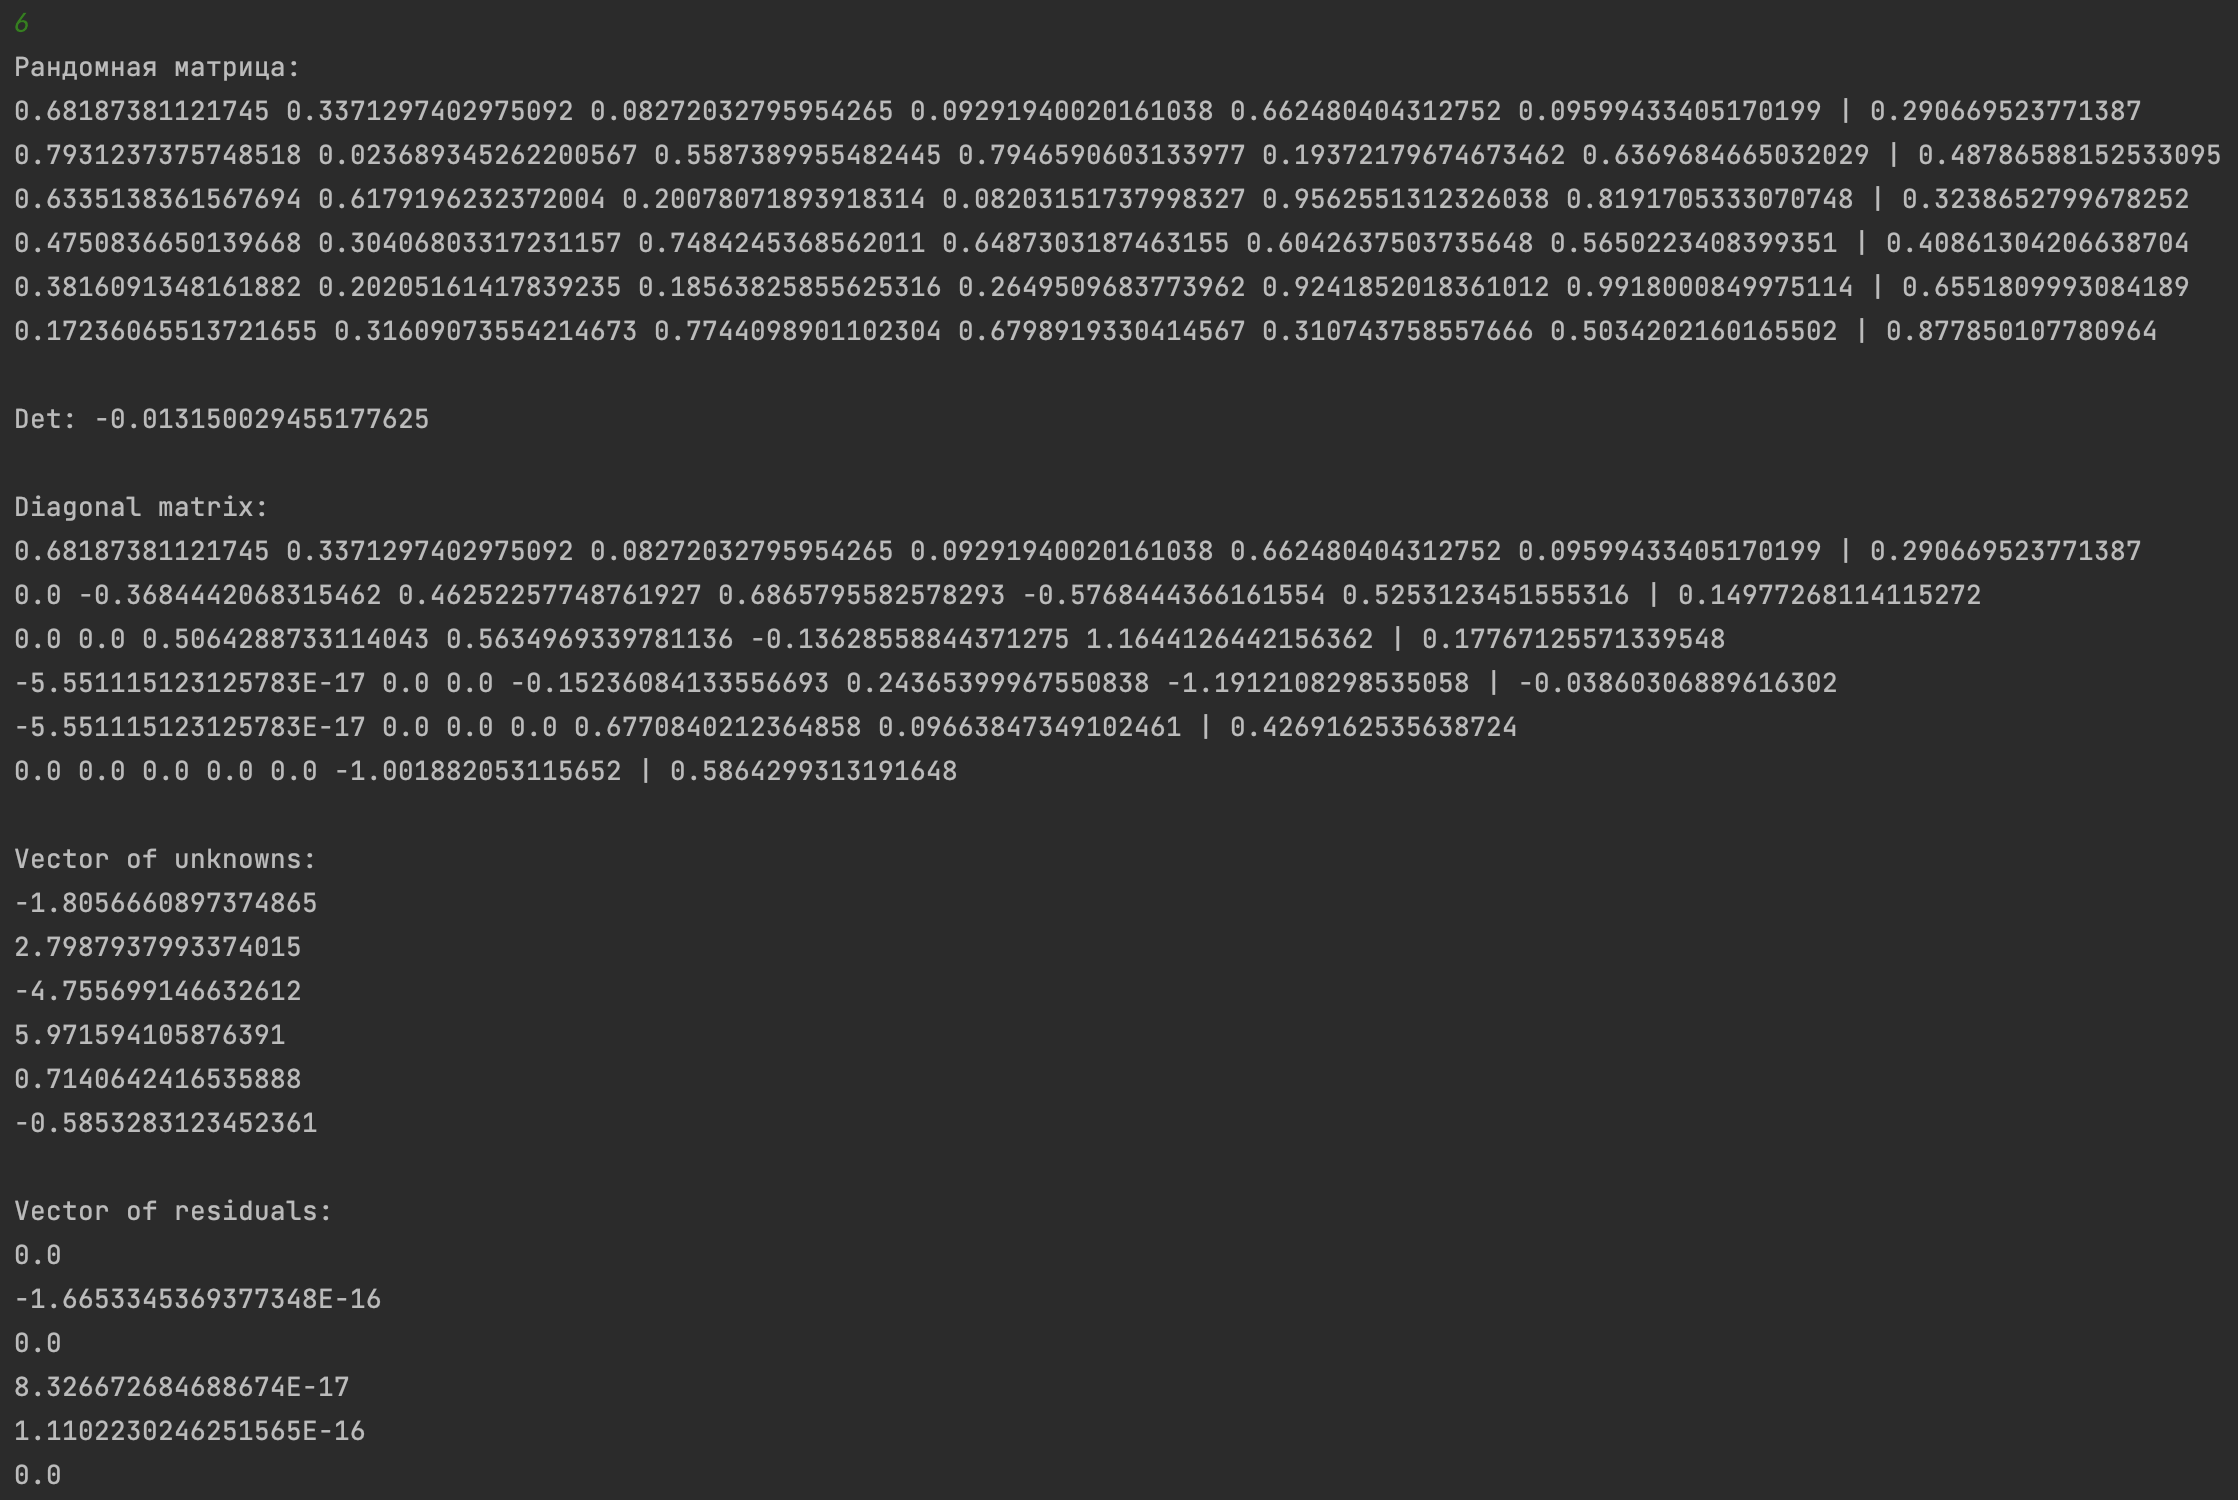
\includegraphics[width=1\textwidth]{3}